\documentclass[article]{jss}

%%%%%%%%%%%%%%%%%%%%%%%%%%%%%%
%% declarations for jss.cls %%%%%%%%%%%%%%%%%%%%%%%%%%%%%%%%%%%%%%%%%%
%%%%%%%%%%%%%%%%%%%%%%%%%%%%%%
%% almost as usual
\author{Tom\'a\v{s} Sieger\\Czech Technical University in Prague \And 
        TODO Second Author\\Plus Affiliation}
\title{Interactive Dendrogram: the \pkg{idendro} Package for \proglang{R}}
%% for pretty printing and a nice hypersummary also set:
\Plainauthor{Tom\'a\v{s} Sieger } %% comma-separated
\Plaintitle{Interactive Dendrogram: the idendro Package for R} %% without formatting
%\Shorttitle{TODO} %% a short title (if necessary)

\newcommand{\myemph}[1]{\emph{#1}}
\newcommand{\Rfunction}[1]{\code{#1}}
\newcommand{\Rfunarg}[1]{\code{#1}}
\newcommand{\mybutton}[1]{\code{#1}}

%% an abstract and keywords
\Abstract{
Hierarchical cluster analysis is a valuable tool for exploring
real-world data. 
We describe an \proglang{R} package \pkg{idendro}, which enables
interactive inspection of the result of hierarchical cluster analysis,
the dendrogram. 
\pkg{idendro} enables to select clusters anywhere in the dendrogram
hierarchy, to zoom and pan the dendrogram, and to visualize the
clustered data not only in a built-in heat map, but also in any
interactive plot implemented in the \pkg{cranvas} package.
}

\Keywords{interactive graphics, visualization, cluster analysis, 
exploratory data analysis, high-dimensional data, \proglang{R}}
%% without formatting:
\Plainkeywords{interactive graphics, visualization, cluster analysis, 
exploratory data analysis, high-dimensional data, R} 
%% at least one keyword must be supplied

%% publication information
%% NOTE: Typically, this can be left commented and will be filled out by the technical editor
%% \Volume{50}
%% \Issue{9}
%% \Month{June}
%% \Year{2012}
%% \Submitdate{2012-06-04}
%% \Acceptdate{2012-06-04}

%% The address of (at least) one author should be given
%% in the following format:
\Address{
  Tom\'a\v{s} Sieger\\
  Department of Cybernetics\\
  Faculty of Electrical Engineering\\
  Czech Technical University in Prague\\
  Karlovo namesti 13\\
  121 35 Prague 2, Czech Republic\\
  E-mail: \email{tomas.sieger@seznam.cz}\\
%  URL: \url{https://nit.felk.cvut.cz/drupal/users/tomassieger}
}
%% It is also possible to add a telephone and fax number
%% before the e-mail in the following format:
%% Telephone: +43/512/507-7103
%% Fax: +43/512/507-2851
%% for those who use Sweave please include the following line (with % symbols):
%% need no \usepackage{Sweave.sty}
%% end of declarations %%%%%%%%%%%%%%%%%%%%%%%%%%%%%%%%%%%%%%%%%%%%%%%



\begin{document}
%% include your article here, just as usual
%% Note that you should use the \pkg{}, \proglang{} and \code{} commands.


\section[Introduction]{Introduction}
%% Note: If there is markup in \(sub)section, then it has to be escape as above.

Modern experiments conducted in many scientific disciplines
often share the common property of producing moderate or
high-dimensional data.
Analysis of such data can be challenging, as we usually need to
consider information from all dimensions simultaneously.
\myemph{Hierarchical clustering analysis} (HCA) (\cite{ESL}) is a
valuable technique giving insight into the structure of such data.
In brief, HCA operates as follows: initially, it considers each
observation to form an elementary cluster, and proceeds iteratively
afterwards: at each stage, it merges two most similar clusters, 
continuing until there is just a single cluster comprising all the
observations. 
The result of such clustering analysis is called the
\myemph{dendrogram}, a tree-like structure depicting the iterative
merging process. To inspect the \myemph{dendrogram}, proper
visualization is needed usually, preferably an interactive one enabling
to focus on particular clusters anywhere in the dendrogram, at any
level of detail.

While HCA can be performed in \proglang{R} easily (e.g. using the
\Rfunction{hclust} function in the \pkg{stats} package), the set of tools
enabling interactive dendrogram visualization is rather limited,
especially when it comes to large data sets.
There exist the low-level dendrogram plotting and interaction
functions \code{plot.dendrogram}, \code{plot.hclust} and
\code{identify.hclust} in the \pkg{stats} package, which, however, can
satisfy basic needs only, as they offer limited interactivity.

%On the other hand, the interactivity offered by \pkg{iPlots}, an
%interactive statistical graphics library written in \proglang{Java},
%is considerable, but large dendrograms can not be inspected in real
%time. % the speed of processing 
%In addition, there are several feature-rich packages offering HCA, but
%none of them allows users to interact with dendrograms and
%(sub)clusters in a convenient way. 

The purpose of this paper is to describe the \pkg{idendro} package, a
fast and interactive dendrogram visualization tool. 
\pkg{idendro} enables to plot large dendrograms, which can be zoomed,
panned and inspected interactively by~selecting and coloring clusters
anywhere in~the~dendrogram hierarchy.
The data clustered can be visualized in a built-in heat map. 
%by using dynamic mutable data frames offered by the
%\pkg{plumbr} package, 
\pkg{idendro} can also be bidirectionally integrated
with any interactive plot implemented in the \pkg{cranvas} package
(e.g. scatter plot, or parallel coordinate plot). 
Such plots can be used not only to visualize the clustered data and
highlight the observations forming the currently selected clusters, but
the user can also brush observations there and see their
correspondence to the structure of clusters revealed by HCA.

\pkg{idendro} is based on \pkg{qtpaint} and \pkg{qtbase} packages.

%In Fig.~1
In the next sections, we will describe the functionality of
\pkg{idendro} on a simple example and TODO....


%%%
%%%
%%%
%\section[Usage]{Usage}
\section[idendro Invocation]{\Rfunction{idendro} Invocation}
%% Note: If there is markup in \(sub)section, then it has to be escape as above.

Let us demonstrate the \pkg{idendro} functionality on the famous
\myemph{iris} data set (\ref{iris}) available from the \pkg{datasets}
\proglang{R} package. The data set consists of 150 observations
of Iris flowers, 50 observations for each of \emph{setosa}, \emph{versicolor}, and
\emph{virginica} species. For each flower, there were 
the~\myemph{sepal length}, \myemph{sepal width}, \myemph{petal length}
and \myemph{petal width} measured (in centimeters)
and stored in~the first four columns of the \myemph{iris} data set. 
The species indicator (coded as a \code{factor}) comes in~the fifth
column.

First, we find clusters in the data using the \code{hclust} function in
the \pkg{stats} package: 

\begin{Code}
    hc <- hclust(dist(iris [, 1:4]))
\end{Code}

Note that we performed HCA on the measurements only, i.e. we excluded
the species indicator from the data.

Next, we want to visualize the dendrogram depicting the~hierarchy 
of~the clusters found. We can simply pass the~result of
\Rfunction{hclust} to \Rfunction{idendro}: 

\begin{Code}
    idendro(hc)
\end{Code}

We get interactive dendrogram drawn. It can be zoomed and panned and 
clusters can be selected in it. However, we can not spot the
correspondence between clusters and the values of individual
observations: which cluster does represent flowers with relatively
short petals, for example? To visualize the values of the observations,
we pass the data set as the second argument to \Rfunction{idendro},
which, by default, enables heat map to be drawn next to the dendrogram
and displays names of the observations next to the heat map:

\begin{Code}
    idendro(hc, iris)
\end{Code}

Now, we get dendrogram drawn with heat map attached to it. This plot
gives quite reasonable insight into which observations form which
clusters. For example, from Fig.~\ref{fig:idendro_window} (which will be
discussed below in full detail) we can see that the top-most cluster
(colored in green) includes flowers with short petals.

Should we want to visualize clusters in feature space in some more convenient 
plot (e.g. a scatter plot), we first need to convert our data to
a~\myemph{mutable data frame} enriched with~special hidden attributes
over~which the dendrogram and the other interactive plot can communicate.
%using the~\Rfunction{qdata} function implemented in \pkg{cranvas}.
%need to
%make such a plot to use the same data as \Rfunction{idendro} does, and
%enable both the plots to communicate over the data, such that the
%observations forming the clusters selected in the dendrogram will get
%selected in the scatter plot automatically. 
%To enable such sharing of our data, we introduce the concept
%of~\myemph{mutable data frames} implemented in~the~\pkg{plumbr}
%package. \pkg{cranvas} leverages this concept in~ the~\Rfunction{qdata} 
%function, which enriches the data with~hidden attributes over~which
%interactive plots can communicate.  
%\pkg{cranvas} is built upon this concept and \pkg{idendro} does so such
%that it can integrate with the great interactive plots offered by
%the \pkg{cranvas} package.
The easiest way to create a \myemph{mutable data frame} from our data is to
simply use the \Rfunction{idendro} return value, because
\Rfunction{idendro} does the conversion
%from regular data frame to the mutable one 
for us:

\begin{Code}
    mdf.iris <- idendro(hc, iris)
    # 'mdf.iris' holds a mutable data frame
\end{Code}

Note that, alternatively, we could have created the~\myemph{mutable
data frame} explicitly, using the \Rfunction{qdata} function of
\pkg{cranvas}, and pass it as the~second argument to \Rfunction{idendro}:

\begin{Code}
    mdf.iris <- qdata(iris)
    # 'mdf.iris' holds a mutable data frame
    idendro(hc, mdf.iris)
\end{Code}

Once we have a~\myemph{mutable data frame} constructed, we can base any
\pkg{cranvas} interactive plot, e.g. to a scatter plot (which gets
automatically linked to the dendrogram):

\begin{Code}
    sp <- qscatter(Sepal.Length, Sepal.Width, mdf.iris, unibrushcolor = FALSE)
    print(sp)
\end{Code}

Now, we can enjoy the bidirectional integration of~\pkg{idendro} with
\pkg{cranvas}. The points in~the~scatter plot get automatically
colored according to~the~currently selected clusters in~the~dendrogram.
Moreover, the~points brushed in~the~scatter plot can be directly
tracked in~so-called \myemph{brushed map} in~the~dendrogram window,
which we describe in the following section.
%because brushing alters the brushed map
%attached to the denrogram and heat map, as such that we can see which
%clusters contain the brushed observations. 

%%%
%%%
%%%
\section[idendro Window Description]{\Rfunction{idendro} Window Description}

\begin{figure}[ht]
\centering
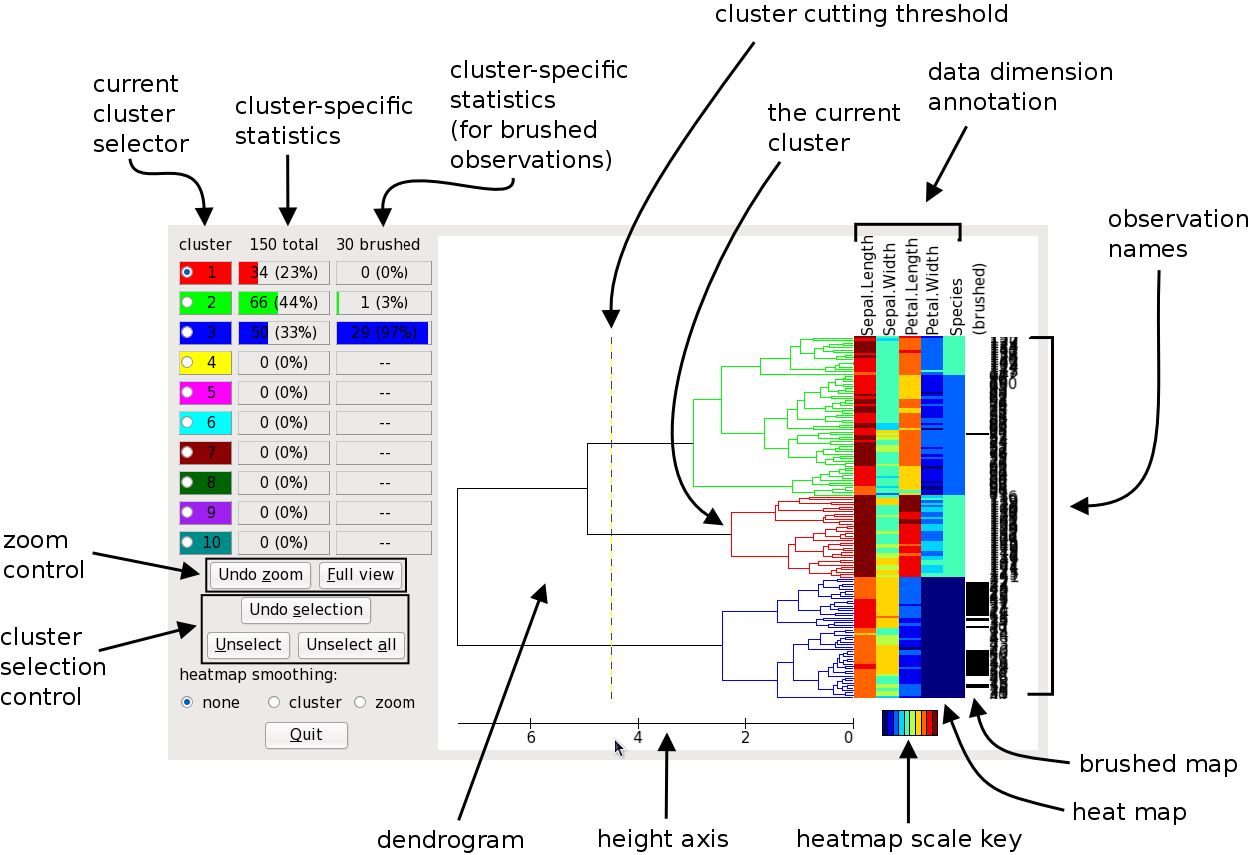
\includegraphics[width=1\linewidth]{pic/idendro}
\caption{\code{idendro} window.}
\label{fig:idendro_window}
\end{figure}

The code given above should result in a plot shown in~ Fig.~1.
We can see a window consisting of two main components: a
simple GUI on the left side and a dendrogram enriched with a heat map and a
brushed map on the right side. 

The top part of the GUI is populated by three
columns: 
\begin{itemize}
\item{current cluster selector, a radio button group determing
which cluster is the \myemph{current cluster},}
\item{cluster-specific statistics telling 
how many observation out of the total number of observations fall in
each cluster, and}
\item{cluster-specific statistics telling how many
observation out of the observations brushed currently fall in each
cluster.}
\end{itemize}

The number of clusters shown in the GUI can be controlled
using the \Rfunarg{maxClusterCount} argument to
\Rfunction{idendro}. 
The colors of the clusters can be controlled using the
\Rfunarg{clusterColors} argument. 

In the bottom part of the GUI there are buttons that help zooming the
dendrogram, selecting and unselecting clusters, and also radio buttons
buttons controlling the heat map smoothing mode. 

On the right side, there is a dendrogram with a heat map and a
brushed map attached to it. 
The dendrogram depicts the hierarchical clustering process, in which,
initially, there were 150 elementary clusters (individual Iris
flowers). Iteratively, at each stage, two most similar clusters got
merged, continuing until there was just a single cluster comprising all
the 150 observations. 
The dendrogram is thus formed by 149 pairs of branches, each pair
representing one merging operation. 
The distance of the two clusters merged at a specific stage is called the
\myemph{height} of the newly merged cluster and can be read from the axis
below the dendrogram.  The first merge operation occured at height
close to 0, while the height of the last (the biggest) cluster is close
to 7.  

The heat map, which is attached to the dendrogram from the right side, comprises
of a row of five colored rectangles drawn next to each of 150 elementary
clusters in the dendrogram (i.e. each observation). The rectangles
code graphically the four measurements made on each Iris flower (i.e.
\myemph{sepal length}, \myemph{sepal width}, \myemph{petal length},
\myemph{petal width}, as shown above the heat map) and the species of
each flower.  
Note that the species were coded as a \code{factor} in~the~data set and
get converted to~ a~numeric type by~idendro internally
such that the~species can be included in~the~heat map.
To compute the color of each rectangle, \Rfunction{idendro}
interpolates the heat map color scale according to data. The heatmap
color scale is shown below the heat map. The scale is defined by the
\Rfunarg{heatmapColors} argument, which defaults to
the blue-green-yellow-red color spectrum.
%The interpolation takes place once, for all values in all dimensions,
%i.e. it is not dimension-specific, such that
%relative differences in some dimension can go unnoticed if data in some
%other dimension are of different magnitude. However, scaling could
%easily be achieved by passing \code{scale}-d version of the data to
%\Rfunction{idendro}.
The heat map appearance is controlled using the \Rfunarg{heatmapEnabled}
argument, which is enabled by default.
The relative size of the heat map %(in respect to the dendrogram) 
can be controlled using the \Rfunarg{heatmapRelSize} argument, 
which determines how
much space is reserved for the heat map out of the space reserved for
both the dednrogram and the heat map. The default is 0.2, i.e. the
heat map takes 20\% and the dendrogram 80\% of their shared space.

The brushed map, displayed immediately next to the heat map, is formed by
white/black rectangles telling whether the coresponding observation
is/is not currently brushed in plots integrated with the dendrogram
(not shown; integration with other plots is decribed in
section~\ref{section:integration_with_other_plots}).
The brushed map is enabled, by default, when there were data passed to 
\Rfunction{idendro}. Brushed map visibility can be controlled using 
the~\Rfunarg{brushedmapEnabled} argument.

The names of individual data observations are displayed on the right side.
They are unreadable in Fig.~\ref{fig:idendro_window}, 
but we will become clear once we zoom-in
the dendrogram. The appearance of the names of the observation can be
controlled using the \Rfunarg{observationAnnotationEnabled} argument, which is
\code{TRUE}, by default.


%%%
%%%
%%%
\section[Interacting with idendro]{Interacting with \Rfunction{idendro}}

\subsection{Cluster selection}

\Rfunction{idendro} enables to select a few clusters in the
dendrogram, label and color them, and provide simple summary statistics
for them. Initially, there are no clusters selected in the
dendrogram\footnote{unless you pass a mutaframe holding cluster
selection metadata in it to \Rfunction{idendro} - see below TODO}.  
To select a cluster, we can either click on a cluster
in~the~dendrogram (on~their top-level branch), or \myemph{cut}
the~dendrogram at~a~specified height.

To select a cluster in the dendrogram manually, we simply click
on~the~top-level branch of~the~cluster. The~cluster gets colored
according to~the~color of~the~\myemph{current cluster} selected
in~the~GUI, and associated with~the~number of~the~\myemph{current
cluster}.  
Initially, the \myemph{current cluster} is the~first one, which is
colored in~red, by default. 
To associate another cluster in~the~dendrogram with the \myemph{current
cluster}, we can simply click on~this other cluster in~the~dendrogram,
which results in~unselecting the~previous cluster and selecting the~new
one. 
To select another cluster while keeping the first one selected, we
simply make the second cluster in the current cluster selector in~GUI
the~\myemph{current cluster}, and pick another cluster
from~the~dendrogram.   

We can also select clusters automatically by \myemph{cutting} the
dendrogram at~a~specified height, i.e. asking \Rfunction{idendro} to
select all clusters merged at or below the specified height. 
To \myemph{cut} the~dendrogram, we move the~mouse pointer below
the~dendrogram axis (it results in~displaying \myemph{cutting}
threshold across the~dendrogram, see Fig.~\ref{fig:idendro_window}) and
press the~left mouse button.  
\Rfunction{idendro} selects all the clusters merged at or below
the~specified height, and associates them with the~first few clusters
in~GUI. 
This is what we see in Fig.~\ref{fig:idendro_window}, in which we
\myemph{cut}
the dendrogram at the height of about 3.7, and obtained three clusters
selected (red, green, and blue ones consisting of 28, 50, and 72
observations, respectively). 

We can see that those three clusters do not reflect the nature
of~the~data, since there were 50 flowers of each  
species. However, we can ask to what extent do the clusters reflect
the natural structure of~the~data? Is the assignment of flowers into
the clusters close to the structure expected, or is it almost random?
Luckily, the heat map can answer this question. When we look at the
last column of the heat map, there is the species of individual flowers
shown, coded numerically (coerced from the levels of the
\myemph{Species} factor). We can see
that the second (as shown in~GUI) cluster (colored in green), which
consists of~50 flowers, matches the flowers of~the~first species
perfectly. 
The first cluster (colored in~red) matches the~second
species almost perfectly - there is only one misclassified flower
in~this cluster. The~third cluster, however, seems to be a~mixture
of~flowers of~the~second and the third species, eventhough
the~subclusters of~this cluster seem to reflect the data structure
quite well. We will get back to studying the structure of the clusters
later when discussing dendrogram zooming and panning.

To unselect the \myemph{current cluster}, i.e. to dissociate the
\myemph{current cluster} shown in~GUI from any cluster shown
in~the~dendrogram, we can click the~\mybutton{"Unselect"} button. To
unselect all clusters, the~\mybutton{"Unselect~all"} button can be
used.  
Selection history is available - the previous selection can be recalled
using the~\mybutton{"Undo~selection"} button.


\subsection{Zooming and panning}

\begin{figure}[t]
\centering
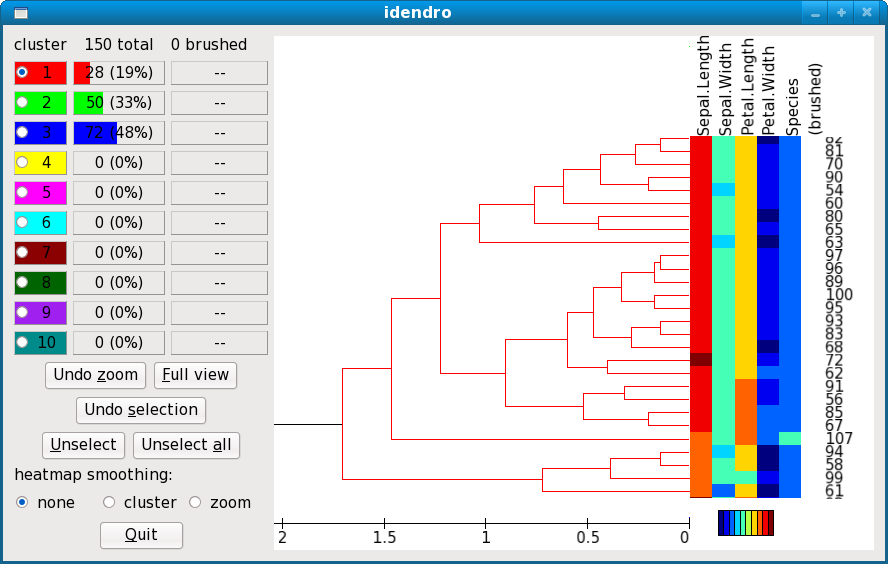
\includegraphics[width=1\linewidth]{pic/idendro_zoomed}
\caption{\code{idendro} window with zoomed dendrogram.}
\label{fig:idendro_zoomed}
\end{figure}

Inspecting the result of~hierarchical clustering analysis usually
involves to iteratively focus on~clusters in~different parts
of~the~dendrogram, at~different nesting levels at~different heights.
For~example, we might want to study the~internal structure of~one
of~a~few top-level clusters, iteratively taking a look deeper and
deeper in~them. 
\Rfunction{idendro} enables such inspection by zooming and panning the
dendrogram. 

To zoom in~the~dendrogram, we can either define a region to zoom to
explicitly, using right mouse click and drag, or using the~mouse wheel.
In~the~latter case, the~amount of zoom can be controlled using
the~\Rfunarg{zoomFactor} argument. 

As~an~example, consider to focus on~the~first (red) cluster
(Fig.~\ref{fig:idendro_zoomed}) and figure out which observation in~this
cluster does not come from~the~same population as~the~rest
of~the~flowers in~it. 
We immediately see that it is the observation 
\#107, which is indeed the most outlying observation in this cluster, as
implied by the dendrogram branch structure.

To restore the~original dendrogram view (i.e. to zoom out maximally),
we can click the~\mybutton{"Full~view"} button.
Zoom history can be recalled by clicking the~\mybutton{"Undo~zoom"}
button. 

Dendrogram can be panned using mouse drag.


%%%
%%%
%%%
\section{Integration with Other Interactive Plots}
\label{section:integration_with_other_plots}

\begin{figure}[t]
\centering
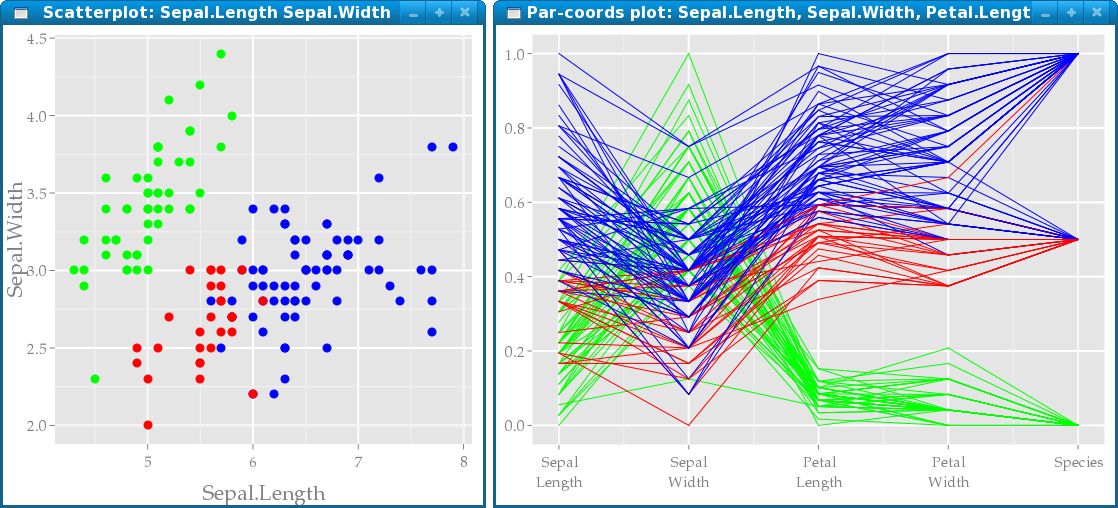
\includegraphics[width=1\linewidth]{pic/cranvas_plots}
\caption{Interactive \code{cravas} plots integrated with \code{idendro}.}
\label{fig:cranvas_plots}
\end{figure}

We keep in mind that %when conducting a~serious data analysis, 
it hardly suffices to look at a~dendrogram and a~heat map alone to
learn what the~data tell us. We usually need to explore more feature space
projections of the data. 
Hopefully, thanks to the effort made by the authors of the \pkg{cranvas}
package,
%which, in turn, is based on dynamic data structures offered by~the~\pkg{plumbr} package, 
\pkg{idendro} can be bidirectionally integrated 
with modern high-speed interactive \pkg{cranvas} plots
(Fig.~\ref{fig:cranvas_plots}). 
We can highlight the~observations forming the~currently selected
clusters there, using the~same colors used to color the~clusters
in~the~dendrogram. 
Moreover, we can also brush observations in~those plots
and, by consulting the~brushed map attached to~the~dendrogram,
we can investigate their correspondence to~the~clusters.

Techically speaking, the integration of \Rfunction{idendro}
with \pkg{cranvas} interactive plots is enabled thanks to~the~concept
of~\myemph{mutable data frames} implemented in the \pkg{plumbr}
package. In brief, \myemph{mutable data frames} are data frames
enriched with hidden metadata (special columns in~the~data frame) that
can be read, written and applications/users can also listen to changes
made to them. 
\pkg{cranvas} leverages the concept of~\myemph{mutable data frames} and
enriches data with metadata controlling color (\code{.color},
\code{.border}), size (\code{.size}) and visibility (\code{.visible})
of~points in~plots. In addition, there is also the \code{.brushed}
column controlling whether given observation is brushed.

\Rfunction{idendro} alters the \code{.color} and \code{.border} 
metadata in~\pkg{cranvas} \myemph{mutable data frames} to color
observations in \pkg{cranvas} plots, and reads the 
\code{.brushed} metadata to learn interactively which observations
are currently brushed in the plots. 

%%%
%%%
%%%
\section{Persisting Cluster Selection}

When inspecting the dendrogram, we might wish to persist the clusters
found so far, such that we will be able to get back to them later. 
\pkg{idendro} introduces two more metadata for this purpose:
\code{.cluster} and \code{.inCurrentCluster}. 
For each observation, \code{.cluster} holds the ID of a currently
selected cluster the observation is member of (or 0, if the 
observation does not belong to any such cluster), and 
\code{.inCurrentCluster} metadata determines whether the observation 
is member of the \myemph{current cluster}. The latter flag can be used
to enable external applications to display the current cluster-specific
information, as shown in the \Rfunction{idendroDemoWithUserCallback.R}
demo.
To persist the currently selected clusters, we can simply remember the
\myemph{mutable data frame} returned by \Rfunction{idendro} (e.g. by
assigning it to some other variable, or saving it to disk).
To recall the persisted clusters, we can invoke \Rfunction{idendro}
passing the persited \myemph{mutable data frame} as the second argument
to it, which results in restoring the persisted cluster selection.
Note, however, that selection history can not be persisted this way.

\section[Case Studies]{Case Studies}
%% Note: If there is markup in \(sub)section, then it has to be escape as above.

\section[Conclusion]{Conclusion}
%% Note: If there is markup in \(sub)section, then it has to be escape as above.


\section[Acknowledgements]{Acknowledgements}
%% Note: If there is markup in \(sub)section, then it has to be escape as above.
The development od the \pkg{idendro} package for \proglang{R} started
as a Google Summer of Code 2012 (\cite{GSoC2012}) project. \pkg{idendro}
was written by Tom\'a\v{s} Sieger and mentored by Catherine Hurley and
Claudia Beleites. This article was written by Tom\'a\v{s} Sieger and
TODO and supported by TODO.

\section[References]{References}
%% Note: If there is markup in \(sub)section, then it has to be escape as above.
\bibliography{refs}


\end{document}

